%harihiom
\documentclass{llncs}

\usepackage[english]{babel}
%\usepackage[utf8]{inputenc}
%\usepackage{amsmath}
\usepackage{graphicx}
\usepackage{float}
%\usepackage{wrapfig}
%\usepackage{titlepic}
%\usepackage[colorinlistoftodos]{todonotes}
\usepackage{graphicx,epstopdf}
\usepackage{amsmath,amssymb,amsfonts,subfigure}
\usepackage{comment}
\usepackage{algorithm}
\usepackage{algpseudocode}
\usepackage{pifont}
\usepackage[normalem]{ulem}
\usepackage[english]{babel}
\usepackage[utf8x]{inputenc}
\usepackage{graphicx}
\usepackage{calc}
\usepackage{graphicx}
\usepackage{subfigure}
\usepackage{gensymb}
\usepackage{natbib}
\usepackage{url}
\usepackage[utf8x]{inputenc}
\usepackage{amsmath}
\usepackage{graphicx}
\graphicspath{{images/}}
\usepackage{parskip}
\usepackage{fancyhdr}
\usepackage{vmargin}
\usepackage{algorithm}
\linespread{1}
\usepackage{color}
\usepackage{cite}
\usepackage{amsmath,amssymb}
\newtheorem{claim1}{Claim}
\usepackage{algpseudocode}% http://ctan.org/pkg/algorithmicx
\usepackage[compatibility=false]{caption}% http://ctan.org/pkg/caption
\setmarginsrb{3 cm}{2.5 cm}{3 cm}{2.5 cm}{1 cm}{1.5 cm}{1 cm}{1.5 cm}

%\newtheorem{theorem}{Theorem}
%\newtheorem{lemma}{Lemma}

\title{Lecture - 2}
\author{Thursday, 28 July 2016 (17:10 - 18:00)}


\institute{Puzzles : The Online Hiring/ Dating Problem}

\begin{document}
\maketitle


\section{Some interesting math jokes and to be thought about questions}

{\footnotesize These paradoxes have not been discussed in detail in the class. They will be covered in the tutorial session.}

\begin{enumerate}

\item A mathematician was caught hiding a bomb in his bag while boarding onto the flight from England to Canada. When asked why he has done so, he says - ``The probability of a man carrying a bomb in a flight = $\frac{1}{1000}$, which is still very high. So I could not have my peace of mind on the journey. But the probability of two people carrying a bomb in the flight = $\frac{1}{1000} \times \frac{1}{1000}\ = \frac{1}{1000000}$, which is very less. So if I carry a bomb, the probability of another bomb being present in this flight reduces by a very big extent."\\
\textit{To think:}What is wrong about these reasoning. 

\item Imagine a very old building standing intact from millions of years. Let $P(today)$ = The probability that this building will fall today and $P(tomorrow)$ = The probability that this building will fall tomorrow. \\
\textit{To think}: Whether $P(today)<P(tomorrow)$, or $P(today)>P(tomorrow)$ or $P(today)=P(tomorrow)$ ?

\item Consider a multiple choice exam conducted countrywide. There are two students- $A$ and $B$. $A$ and $B$ both have got equal marks. But $A$ knew the answers correctly of the questions he answered, while $B$ answered the questions randomly and was lucky enough to get the same marks as $A$. \\
\textit{To think:} By looking at their OMR\footnote{Optical Mark Reading- One where we darken the bubbles corresponding to the correct answer- A/B/C/D.} sheets, can you tell, which is the sheet of $A$ and which is the sheet of $B$.

\end{enumerate}


\section{Online Hiring/ Dating Problem}
\textbf{Problem Statement}: You are searching for a match for marriage. There are $1000$ boys standing in a row, and you have to choose one out of them. According to the rules of the game, you can interview the boys only in a sequence one by one. If the sequence is : \\ $B_1\ B_2\ B_3\ B_4\ B_5\ ....... \ B_{1000}\ $, you will first see $B_i$, only then $B_{i+1}$. You have a choice to accept or reject a boy. If you accept one, the game gets over and you tie a knot with the selected individual. If you reject a boy, you can not return back to him. He is gone forever. What should be the optimal strategy to choose as best person as possible?  

\textbf{Solution:} \\
\textit{Intuition:} Check out on some people. This will give you an idea of what the crowd is like. After getting the idea of the crowd, it will be easier to choose the best person. \\

Look for the first $k$ boys. Let $B_k$ be the best among these. Reject all of these $k$ boys and keep a note of $B_k$. After k boys, as soon as you see a boy better than $B_k$, you accept. This has been shown in Figure \ref{boy}.

\begin{figure}[h]
\centering
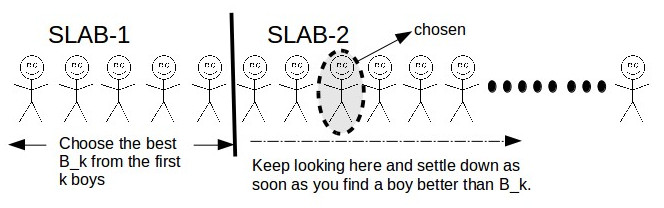
\includegraphics[width=0.9\textwidth]{boys.jpg}
\label{boy}
\caption{The technique to choose as best boy as possible}
\end{figure}

As an intelligent reader can make out, the value of $k$ plays a significant role here. If the value of $k$ is very small, you will end up choosing an inferior quality boy, since you have not seen enough samples. If $k$ is very big, not enough boys will be left in slab 2 to take a proper decision. So, now we look at the question - What should be the value of $k$.\\

Let $f(k)$ denote the quality of the selected boy when the first $k$ boys are employed as the sample of the entire population of available choices. We can plot a curve with $k$ on the X axis and $f(k)$ on the Y axis\footnote{Try writing a piece of code and observe how this plot looks like}. The roots of the equation $f'(k\ =0)$ give us the value of $k$ for which $f(k)$ is maximum, or in other words, we get the highest quality boy. This has been explained in detail in Algorithm \ref{dating}.

\begin{algorithm}
\caption{The Dating Algorithm}\label{dating}
\begin{algorithmic}[1]
\Procedure{Dating}{}
\State \textbf{Input}:- Array of the quality of $n$ boys $A[1,2,.....,n]$, $A[i]$ represents the quality of the $i_{th}$ boy, $k$
\State \textbf{Output}: $A[Best]$- The quality of the solution, $Best$- The index of the selected boy.
\State $Best\ = 0$
\For {$i\ =\ 1\ to\ k$}
\If {$A[Best] < A[i]$}
\State $Best \gets i $
\EndIf
\EndFor
\For {$i = k+1\ to\ n$}
\If {$A[Best] < A[i]$}
\State $Best \gets i$
\State break
\EndIf
\EndFor
\State return $Best$, $A[Best]$
\EndProcedure
\end{algorithmic}
\end{algorithm}

\subsection{Probability that Algorithm \ref{dating} fetches you the best boy}

The algorithm fails to fetch the best boy when one of the following two events occur.
\begin{itemize}
\item When the best boy is in the first $k$ boys(Our sample of the crowd). It is because, according to the algorithm the first $k$ boys are rejected and hence the best boy will also be rejected.  
\item When we pick a boy after the first $k$ boys and he is non-best. This is shown in Figure \ref{hero}. Here, we end up picking a suboptimal boy which is sandwiched between the $k+1_{th}$ location boy and the best boy. 
\end{itemize}

\begin{figure}[h]
\centering
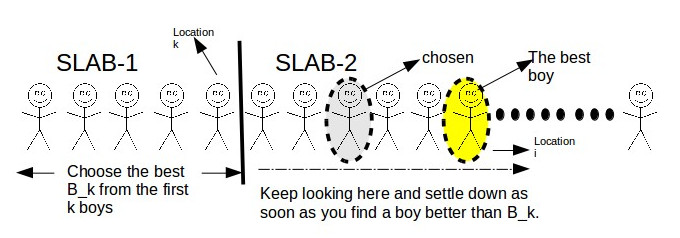
\includegraphics[width=0.9\textwidth]{hero.jpg}
\label{hero}
\caption{Choosing someone who is not the best}
\end{figure}

$Pr$(Best boy is in the first $k$ locations) = $ \frac{k}{n}$, since there are $k$ ways in which the best boy can be present at any of the first $k$ locations and the total number of locations to be present at are $n$. \\

We call a boy to be the pseudo-best if its quality is greater than $B_k$ and lesser than the quality of the best boy.
 
For the algorithm to fetch the best boy
\begin{enumerate}
\item The best boy should be present after the first $k$ locations. 
\item If the location of the best boy is $i$, no pseudo-best boy should be picked from the locations $[k+1,i-1]$.
\end{enumerate}


Hence, $Pr$(We get the best boy)= $Pr$(Best boy is at the location $i$ and no pseudo-best boy is present in the location $[k+1,i-1]$ ).\\

Given a location $i$, $Pr$(Best boy is present at this location) = $1/n$. \hspace{2mm} ....(1)\\

$Pr$(Pseudo-best boy is not there at locations $[k+1,i-1]$) = $\frac{k}{i-1}$. \hspace{2mm} ...(2) 

Why? Let us see.\\ 
We now, divide the queue of boys in three slabs as shown in Figure \ref{slabs}.

\begin{figure}[h]
\centering
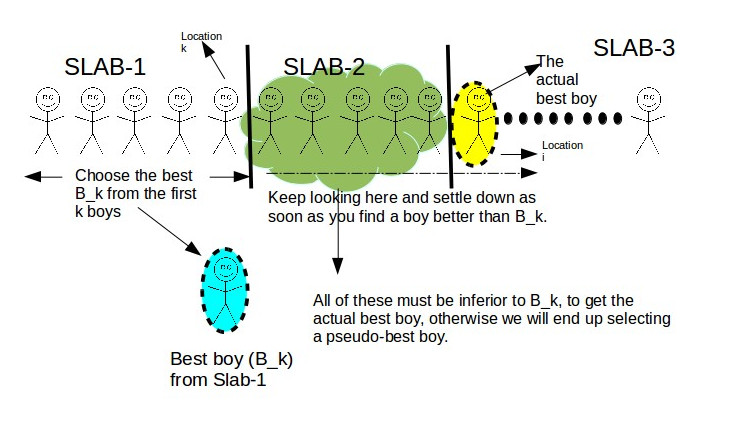
\includegraphics[width=0.9\textwidth]{slabs.jpg}
\label{slabs}
\caption{Choosing the best}
\end{figure}

$Pr$(The best boy from locations $1$ to $i-1$ is present before the location $k+1$)= $\frac{k}{i-1}$

From (1) and (2), \\
$pr$(winning when the best boy is at the location $i$) = $\frac{1}{n} \times \frac{k}{i-1}$\\

Now the location of the best boy can vary from $k+1$ to $n$. We have to take all these cases in account. \\

$Pr$(We end up choosing the best boy)= $\sum_{i=k+1}^n \frac{1}{n} \times \frac{k}{i-1}$\\

= $\frac{k}{n} \sum_{i=k+1}^n \frac{1}{i-1}$\\

= $\frac{k}{n} \sum_{i=k}^{n-1} \frac{1}{i}$\\

= $\frac{k}{n} \int_{k}^{n} \frac{1}{i} di$ (we replaced $n-1$ by $n$ assuming $n$ is a very large number)\\

= $\frac{k}{n}|log\ i|_{k}^{n}$\\

=$\frac{k}{n} (log\ n - log\ k)$\\

\[
 \boxed{f(k)\ =\ \frac{k}{n} (log\ n - log\ k)}
 \]
 
 Differentiating \\
 
 $f'(k)=\ \frac{1}{n} (log\ n\ -\ log\ k) + \frac{k}{n} \times \frac{-1}{k}$\\
 
 Equate to $0$. \\
 
 $\frac{1}{n} (log\ n\ -\ log\ k) + \frac{k}{n} \times \frac{-1}{k}\ =0$\\
 
 $ (log\ n\ -\ log\ k\ -\ 1\ = 0)$\\
 
 or, $log\ n\ -\ log_e\ e\ =\ log\ k$\\
 
 or, $log\ \frac{n}{e}\ =\ log\ k$\\
 
 or, 
\[
 \boxed{k=\ \frac{n}{e}}
 \]


\end{document}

